\chapter{Appendix F: Extra Plots and Figures}
\label{AppendixF}

\section{SOBOL Analysis With Washin and Washout}
\label{sec:AppendixF:sobol_analysis_with_washin_and_washout}
\subsection{Final Value Analysis}
\subsubsection{Resources}
Despite the resource consumption rate directly depending on $e, v$ and $K$, the parameters had very little influence on the final value as evidence by the ST and S1 bar being near 0. 
The resource population was mainly driven by the washin and washout value. 
The peak resources are driven completely by the washin rate. 
Not many interactions between two or more parameters were occurring. 

\subsubsection{Phages}
The most important factor for the final phage value is $r$, followed by $\beta$ and $\omega^o$. 
The other parameters had little to no effect on the final phage value. 

\subsubsection{Total Bacteria}
The sum of uninfected and infected bacteria depended heavily on higher order interactions as $ST_i \gg S1_i$. 
Although not shown, the bar plots for the total bacteria resembled that of the bar-plots for the uninfected bacteria, and less that of the infected bacteria. 

\subsection{Peak Value and Time of peak}
To create the custom SOBOL analyses, the peak value and the time at the peak of the population is measured and analyzed. 
The peak is defined as the point where the population reaches 95\% of its absolute maximum value. 
The time at peak is measured at the point in time that the population reaches 95\% of the maximum value. 
This removes unintended side effects of the simulation. 
For populations that are only increasing in value, this prevents the measured peak from bunching up at the end of the simulation, skewing the data. 
As the peak is defined at 95\% of the absolute maximum value, populations that have a faster increase on population count at the end will have a time value closer towards the end of the simulation. 
For populations that reach a plateau, the 95\% rule will push the peak time towards the beginning of the simulation, while still "respecting" the absolute final value since $95\% \approx 100\%$. 
The 95\% rule can fail under certain situations, such as when there is cyclic behavior. 
See \nameref{sec:appendixF:why_95} for a more detailed explanation on why the 95\% rule is used. 


The results of the SOBOL peak and time at peak analyses can be seen in \Cref{fig:created:SOBOL_peak} and \Cref{fig:created:SOBOL_peak_time}. 
Although some of the bars between the final, peak, and time at peak values are the same, some are different. 
But overall, similar values can be seen across the the final, peak, and time at peak analyses. 
The peak infected values are more certain compared to the final infected values, which could be due to the 95\% rule removing some of the noise of the simulation. 
The time at peak values have less error compared to the final and peak value. 
This is due to the restricted range of values. The time at peak value can only fall somewhere between 0 and 15, the start and end values of the simulation respectively. 
The final and peak values can fall anywhere between 0 and any value, depending on the IC and how high the population can rise, and how fast the population can fall, \textit{if} the population count falls. 

\begin{figure}[ht!]
    \centering
    \begin{subfigure}{0.32\linewidth}
        \centering
        \captionsetup{width=1\linewidth}
        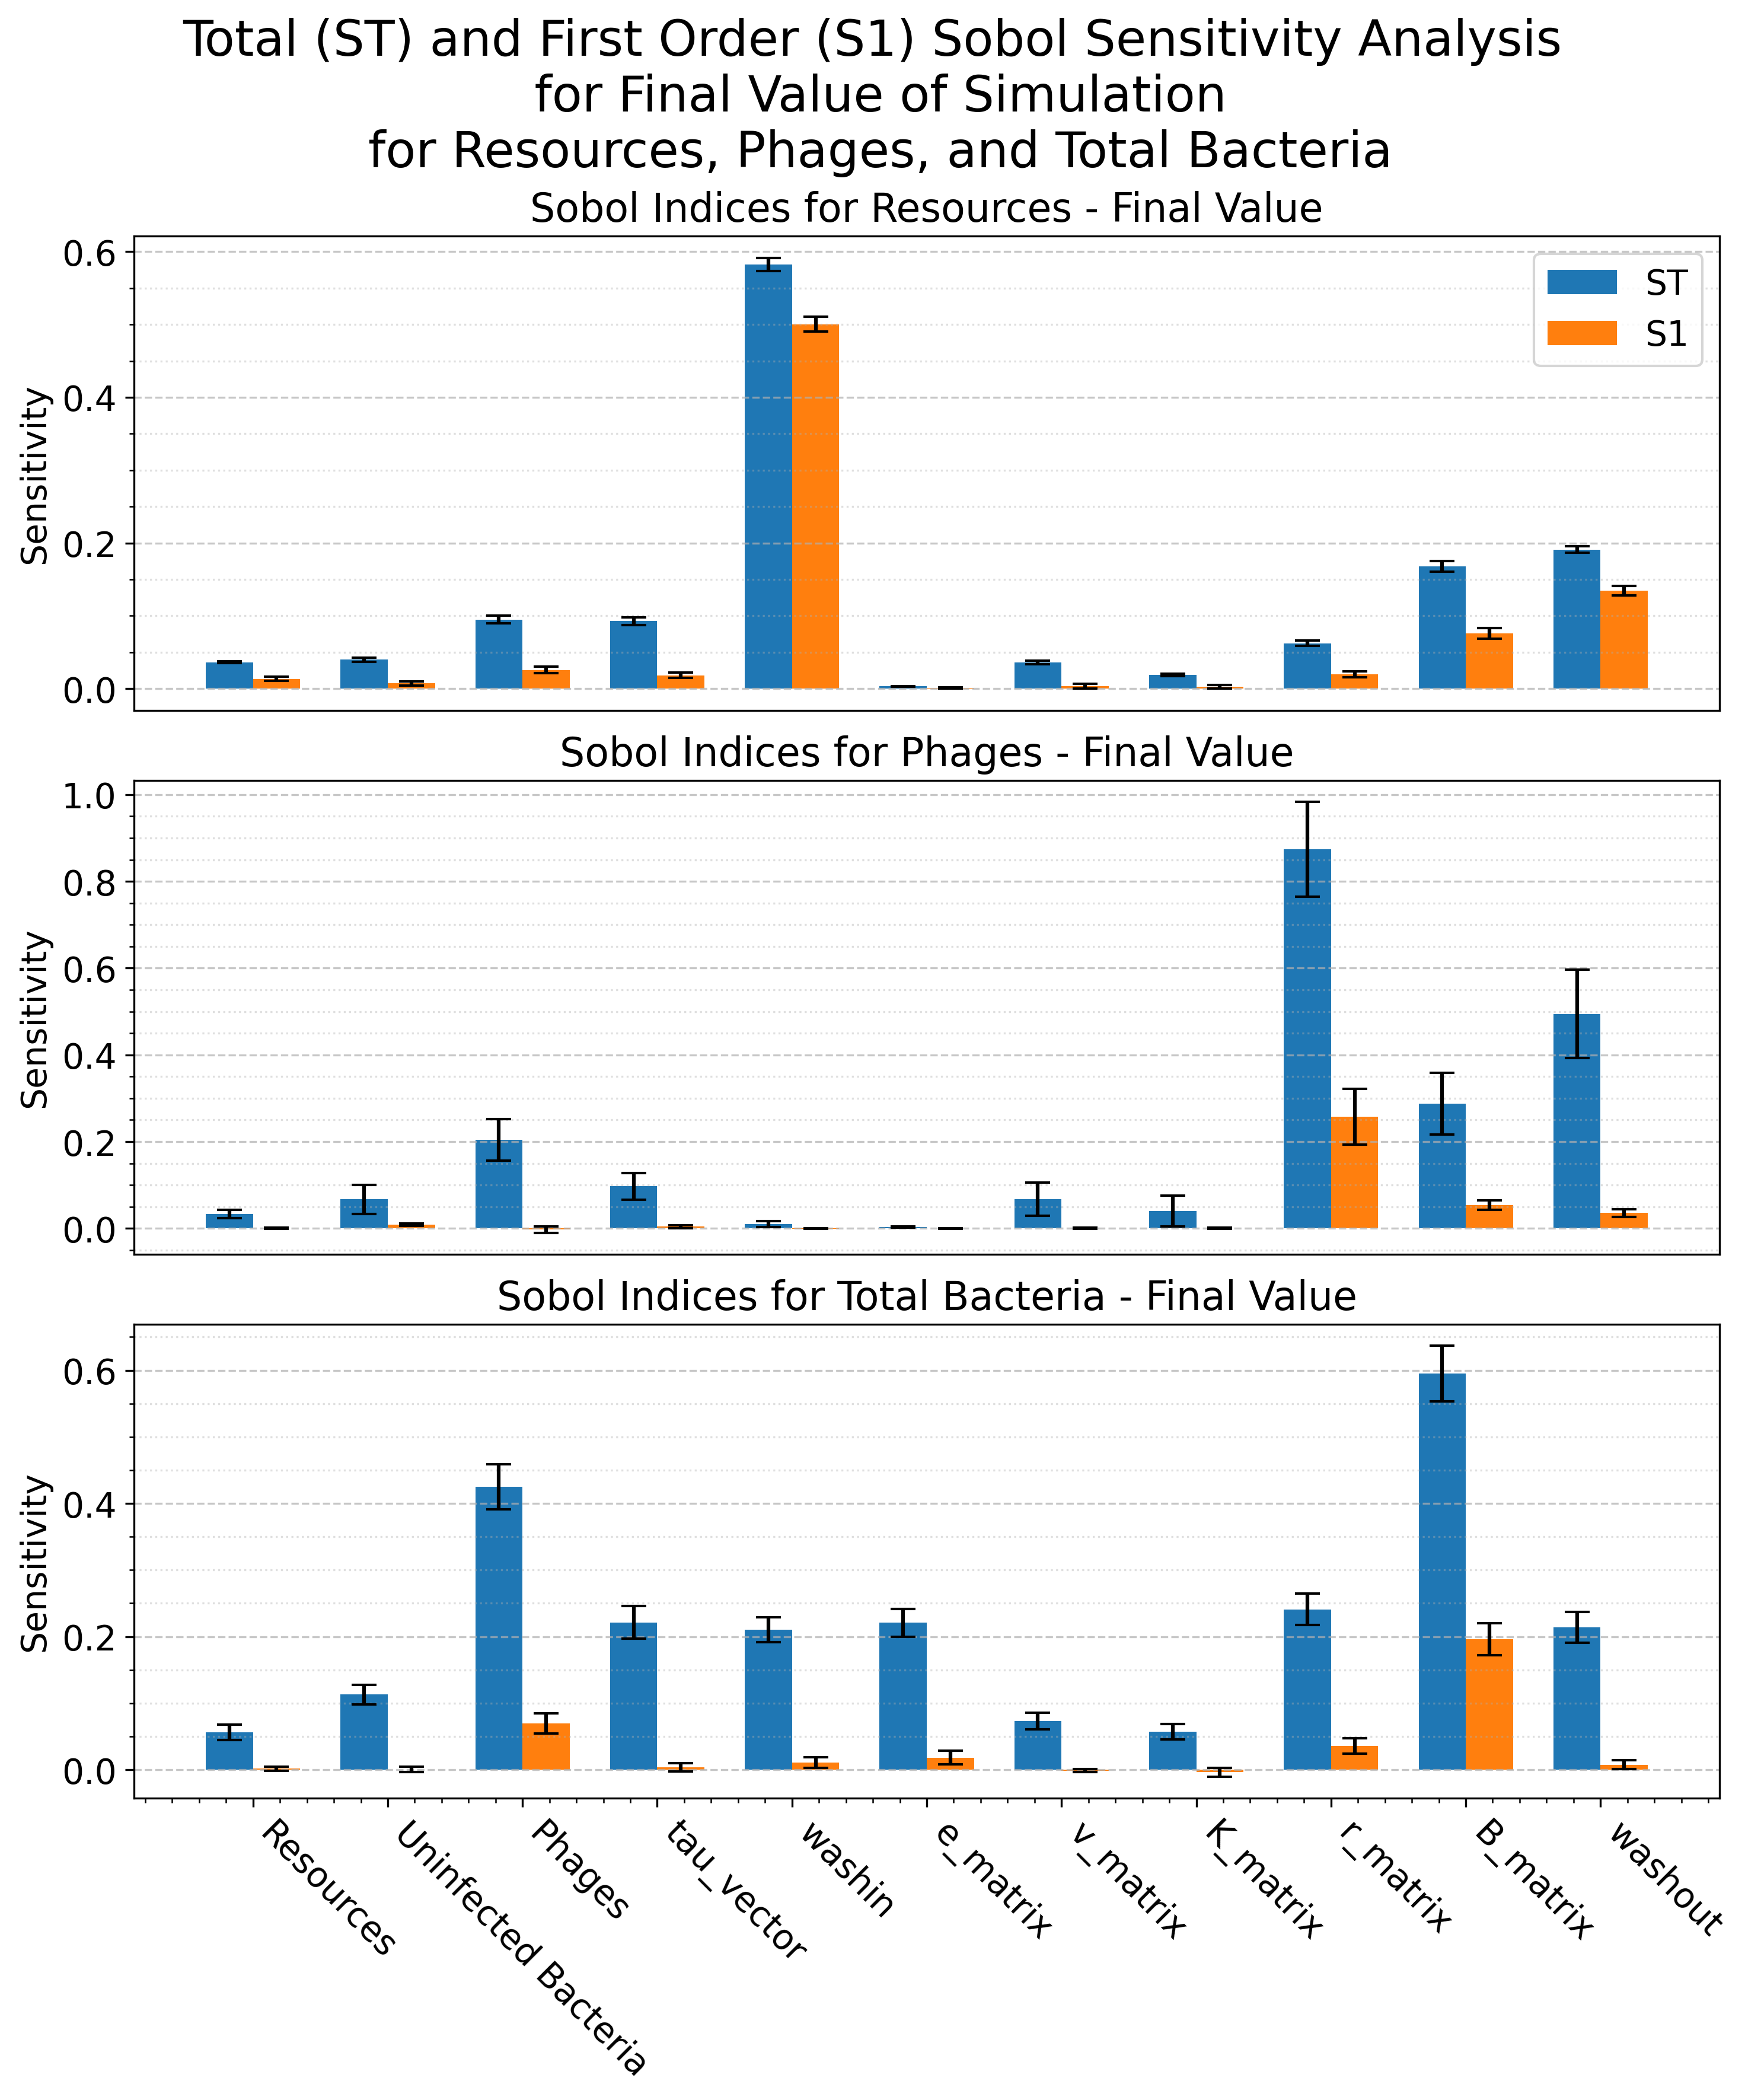
\includegraphics[width=\linewidth]{Plots/Created/SOBOL/SOBOL_analysis_1749149674_Final.png}
        \caption{
            Final population value. 
        }
        \label{fig:created:SOBOL_final}
    \end{subfigure}
    \hfill
    \begin{subfigure}{0.32\linewidth}
        \centering
        \captionsetup{width=1\linewidth}
        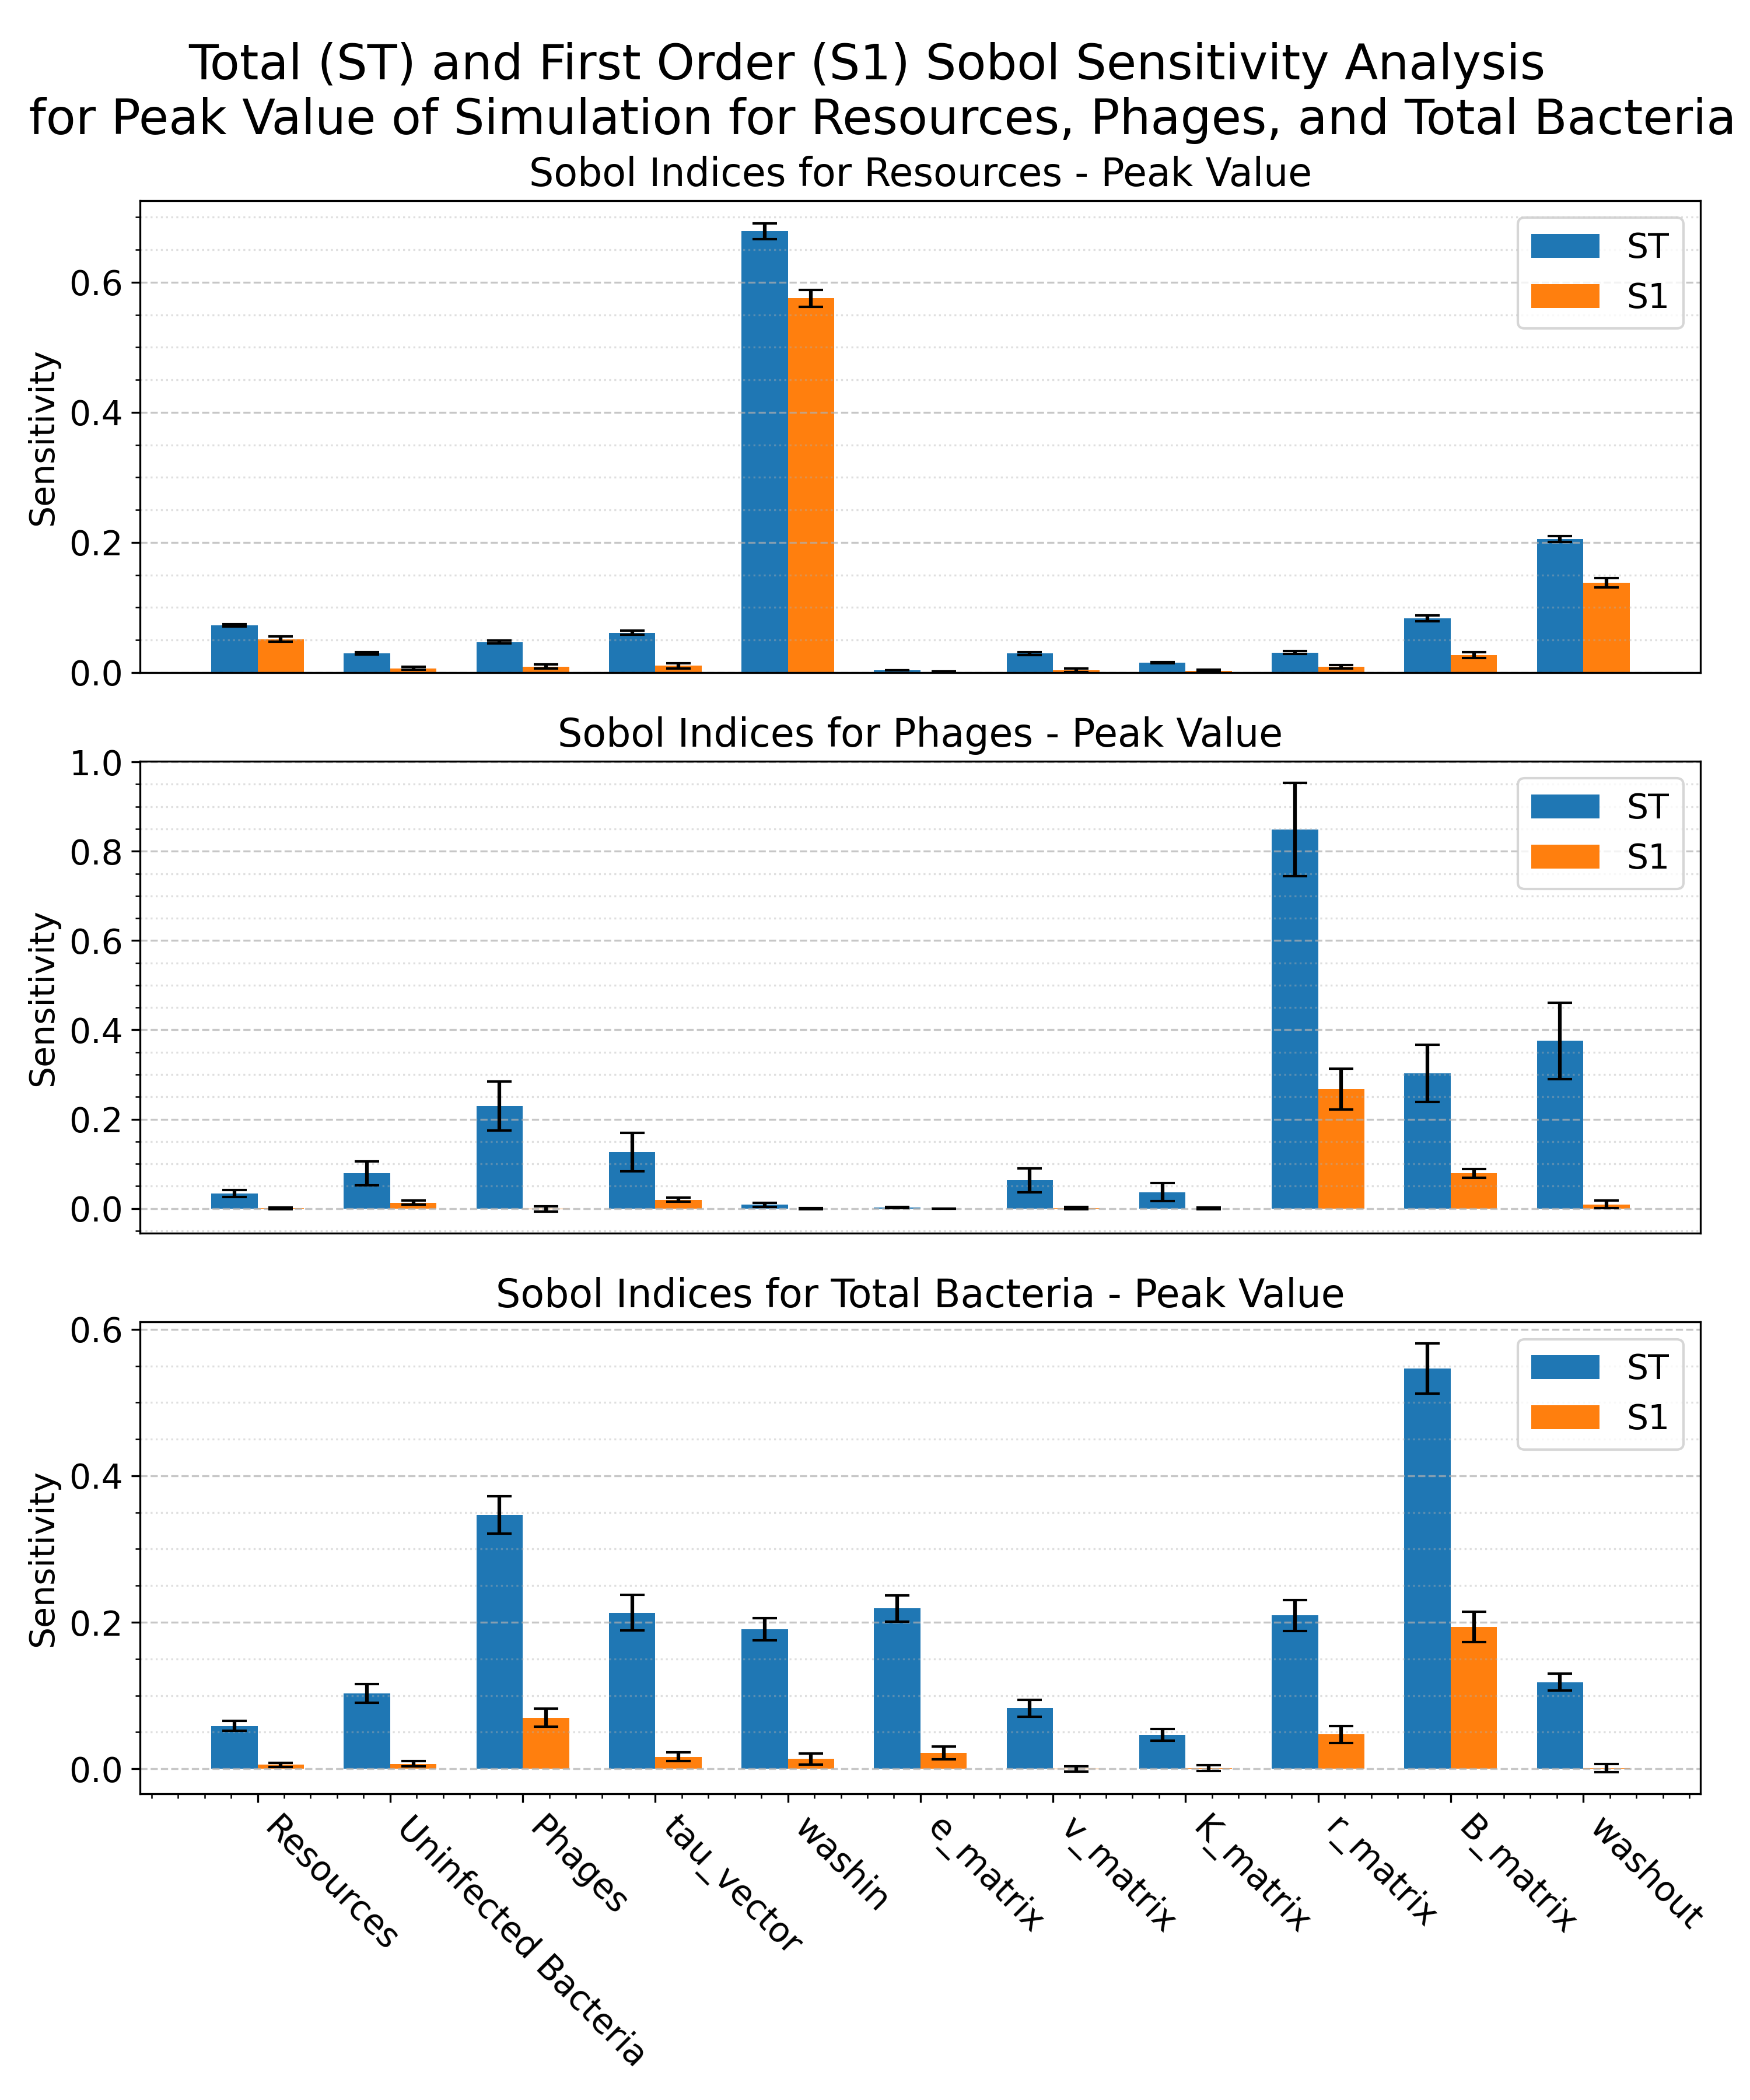
\includegraphics[width=\linewidth]{Plots/Created/SOBOL/SOBOL_analysis_1749149674_Peak.png}
        \caption{
            Peak population value. 
        }
        \label{fig:created:SOBOL_peak}
    \end{subfigure}
    \hfill
    \begin{subfigure}{0.32\linewidth}
        \centering
        \captionsetup{width=1\linewidth}
        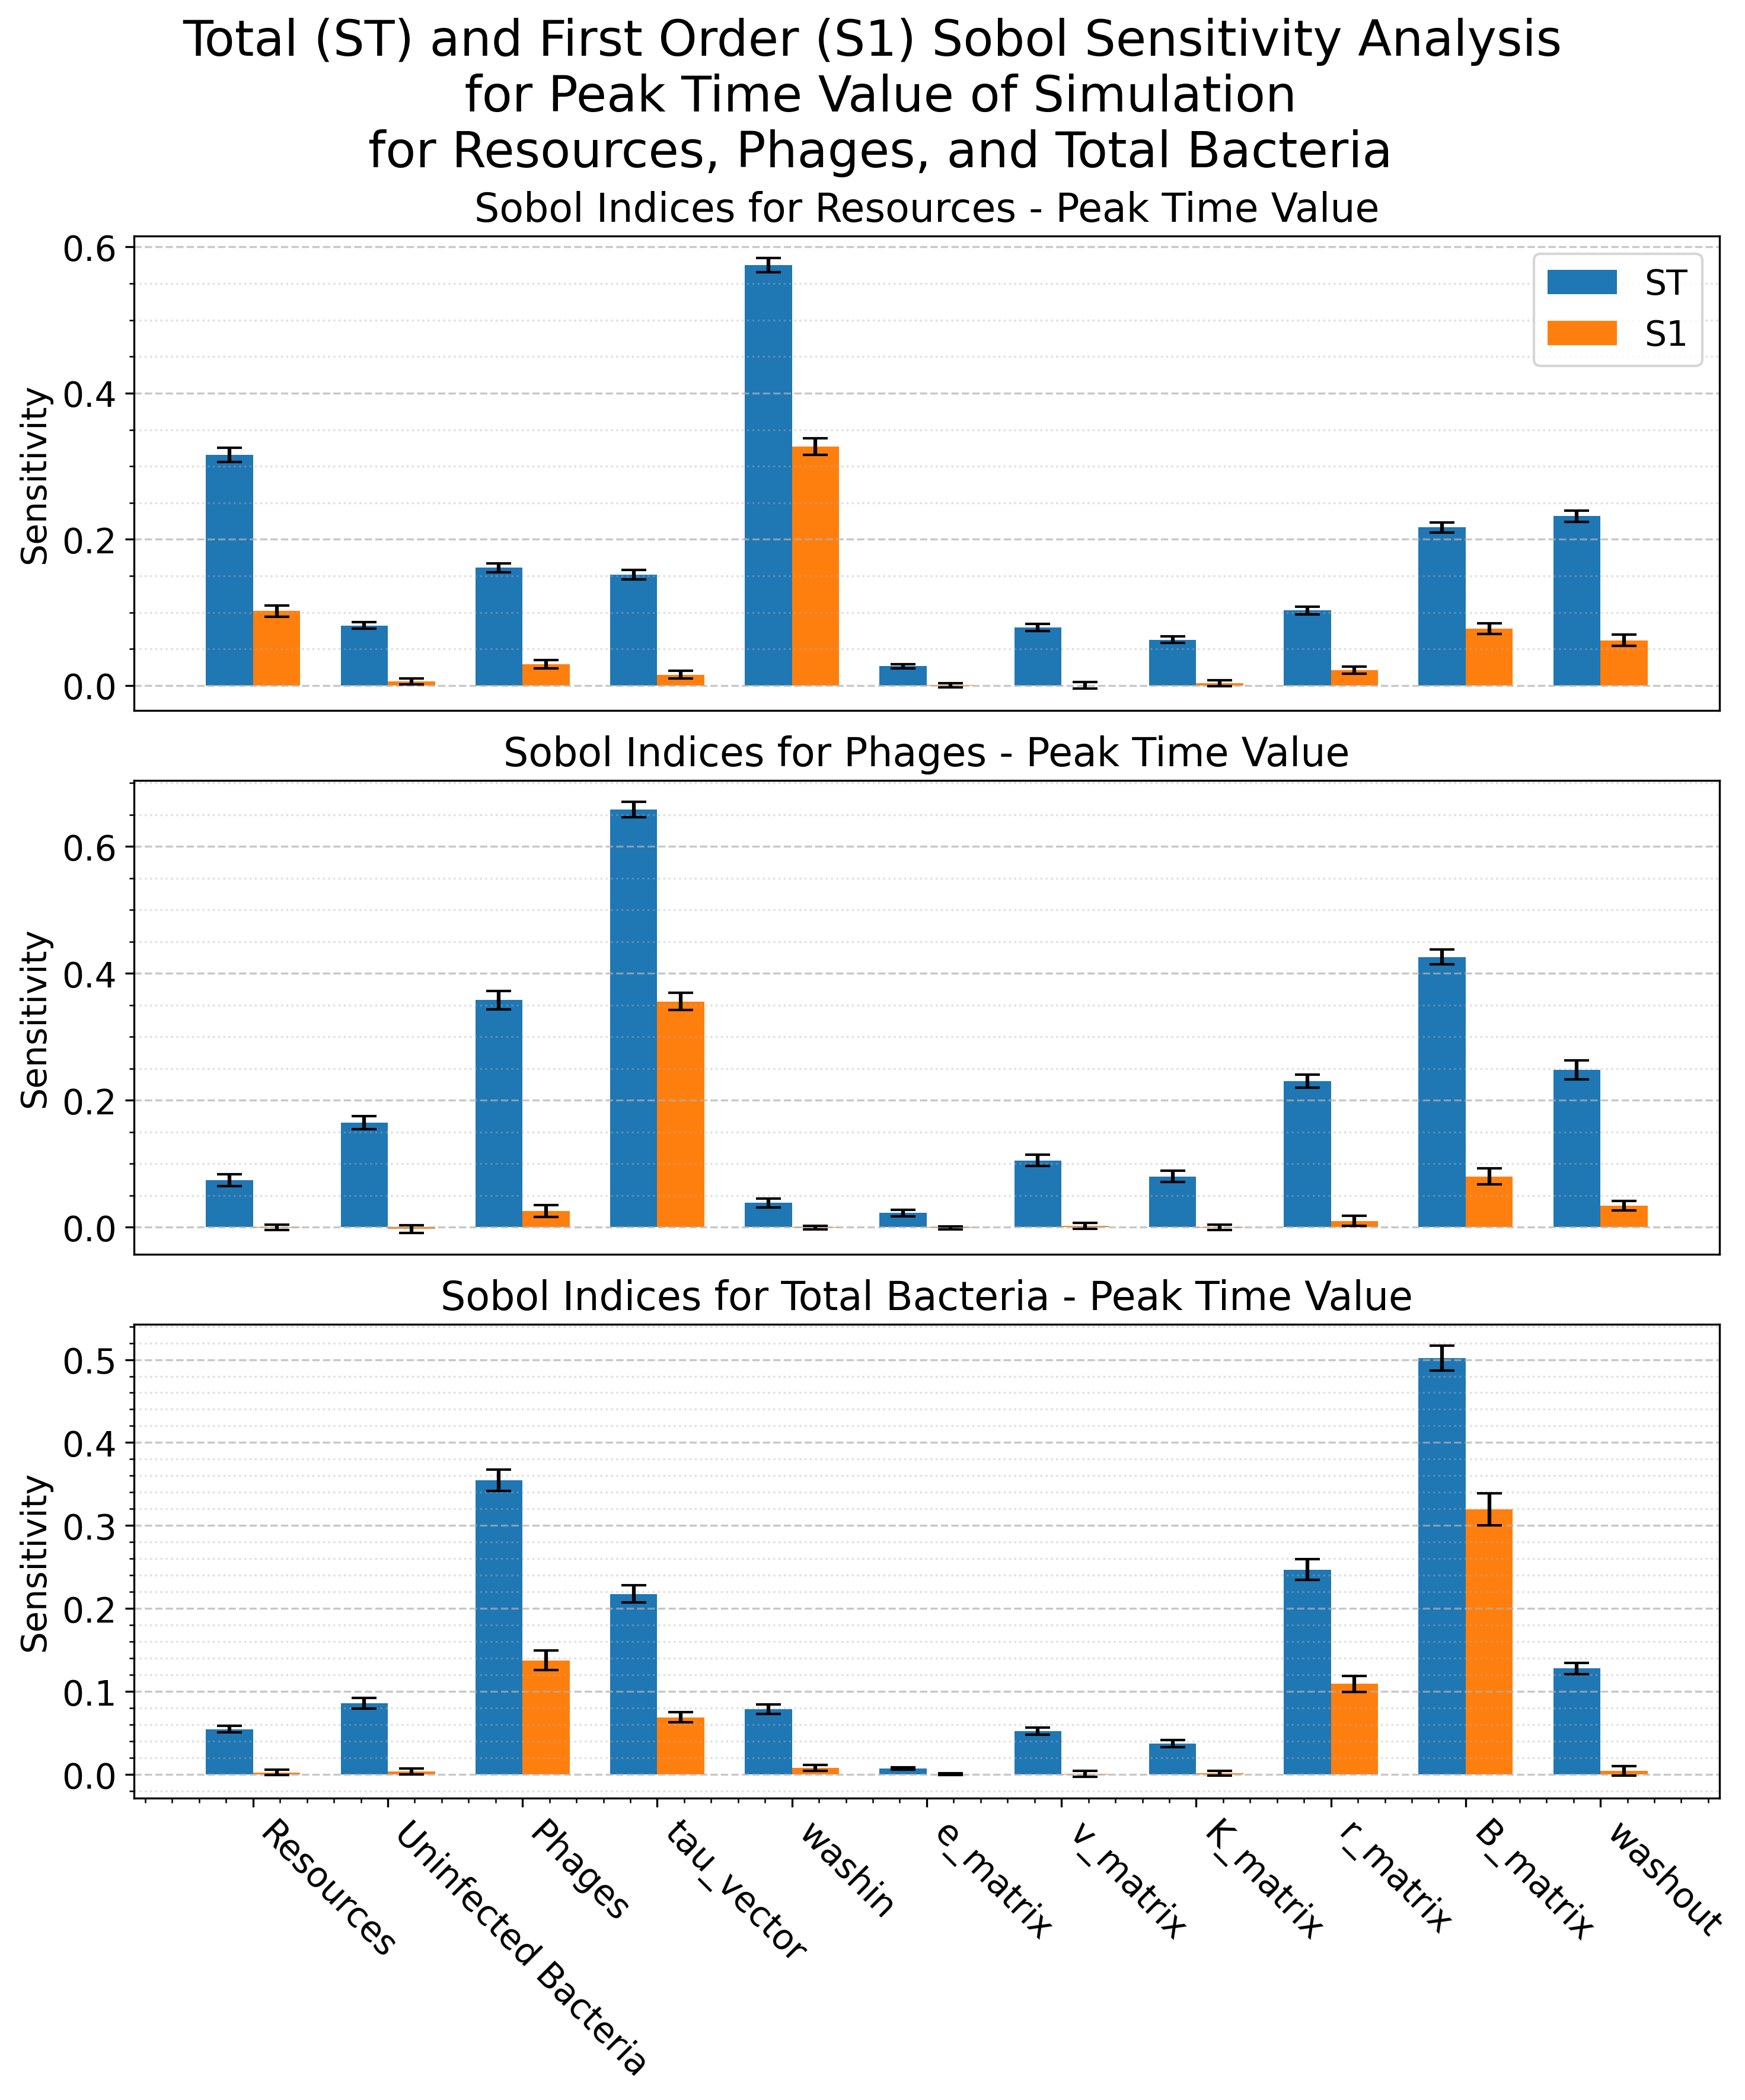
\includegraphics[width=\linewidth]{Plots/Created/SOBOL/SOBOL_analysis_1749149674_Peak_Time.png}
        \caption{
            Time at peak population. 
        }
        \label{fig:created:SOBOL_peak_time}
    \end{subfigure}
    \caption{
        SOBOL analyses for the final, peak, and time of peak value with a washin and washout rate. 
        The data was saved from the dashboard and plotted using Matplotlib. 
        The values used for this SOBOL test can be found in \Cref{tab:appendixE:SOBOL_analysis_values}. 
    }
    \label{fig:created:SOBOL_analyses}
\end{figure}

\section{Why 95\%? }
\label{sec:appendixF:why_95}
The 95\% rule helps in the IVA analysis. 
Due to the solver, when taking the absolute peak value, the same time value can occur. 
Or in an ever increasing value like phages, the peak values occur at the last time step of the simulation, or plateaus and doesn't grow anymore. 
However, as the parameter value is changing, each graph for every input change will change the growth rate of the agent, changing how fast the agent population grows. 

\Cref{fig:appendixF:IVA_95_vs_100} shows how using the 95\% rule vs the 100\% rule for finding the max value reached helps smooth out computational errors from the ODE solver and smooths out the shape. 
For the phages, using the 100\% rule (\Cref{fig:appendixF:IVA_phages_100}) shows that the population peaked at the end of the simulation, $t=15$, for all $e$ values. 
However at $t=15$, the population plateaued, as evident by the line graph. 
Plotting the same plot, but calculating the peak at 95\% of the actual peak (\Cref{fig:appendixF:IVA_phage_95}) shows that the green line ($e=0.25$) "reached" its peak at $t=8.4$ before the red line ($e=0.05$) at $t=9.4$, a full unit of time after $e=0.25$. 
The user can thus conclude that for this instance, larger $e$ values will cause the phage population to reach its "peak" faster than smaller $e$ values. 

\Cref{fig:appendixF:IVA_uninfected_bacteria_95} and \Cref{fig:appendixF:IVA_uninfected_bacteria_100} likewise show how the 95\% rule can improve analysis of the change in peak time. 
\Cref{fig:appendixF:IVA_uninfected_bacteria_100} shows how apparently the peak is reached at set time values. 
Due to how \textit{solve\_ivp()} from SciPy works, it automatically chooses time values that it thinks would best capture the dynamics of the system without calculating too many steps. 
The user can control the step size by decreasing the absolute and relative error bounds, as well as by minimizing the time steps. 
The user can also provide their own time range with the number of steps to run, increasing the control of the time values chosen. 
It takes about 0.02321 seconds to run a simulation for 15 time units, where 200 time steps are selected and solved by the solver. 
Comparatively, a simulation with 1000 time units and 1000000 (a 5000x increase in samples) equidistant time samples takes about 1.71651 seconds to run, a 73.95562258x increase in time spent computing the simulation. 
The total time taken to run the whole method call, a call to the simple graph maker at the top of the dashboard took 1.76130 seconds vs 17.70634 seconds. 



Alternatively instead of controlling the solver, the user can use the 95\% rule.
Although some accuracy is lost. 
Going from the 100\% rule to the 95\% rule, the solver still captures the peak values and the dynamics, but the accuracy is lost. 
The 100\% rule shows that for $e=0.25$, the time the uninfected population reached its peak occurred at $t=3.2$. 
But for the 95\% rule, the time at which the peak occurred at is at $t=3.05$. 
The slope (the $a$ value) and the intercept (the $c$ value) are somewhat similar, with very high and similar $R^2$ values (0.97), suggesting a good linear fit of the data. 

\Cref{fig:appendixF:IVA_uninfected_bacteria_100_own_time} shows how the by increasing the time sampling to more fine grained results in a more accurate graph. 
Instead of having the solver choose the time values to test, 1000 equidistant time values were selected between 0 and 15. 
The solver can more accurately calculate the population values and calculate the proper peak time. 
Comparing the 100\% rule without the custom time values with the 100\% rule with the custom time values shows the same time values were calculated. 
in both, the $e=0.25$ resulted in a time of peak at 3.2 and for $e=0.05$, the time of peak occurred at $t=3.95$. 
This is in stark comparison to the 95\% rule vs 100\% rule without the custom time, showing a difference of $0.15$ time units. 
The custom time values also preserved the shape of the curve $e$-value vs time curve, being almost identical to that of the 95\% rule as seen in \Cref{fig:appendixF:IVA_uninfected_bacteria_95} and \Cref{fig:appendixF:IVA_uninfected_bacteria_100_own_time}. 

Another issue that arises with the custom time is that it doesn't solve the issue seen with the phages, where the time of peak is at $t=15$. 

The user can control the \% rule with a value input on the dashboard. 
They can select to use the 95\% rule, or 100\% rule, or even 83\% rule if they want by changing the value they use. 
The user can use their own custom time values, to ensure that they get high quality curves. 

\begin{figure}
    \centering
    \begin{subfigure}{1\linewidth}
        \centering
        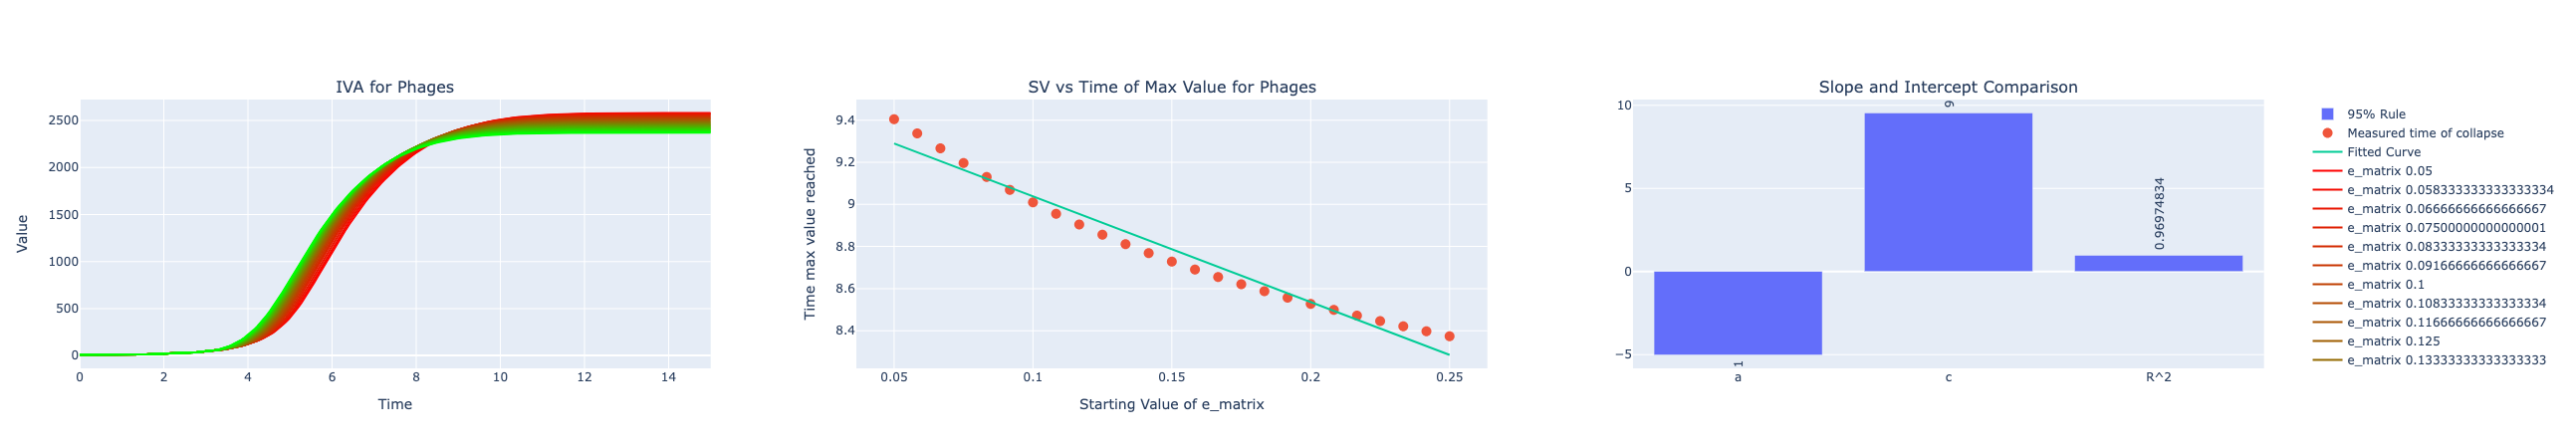
\includegraphics[width=\linewidth]{Plots/Created/IVA/initial_value_analysis_Phages_95.png}
        \caption{
            IVA for phage population, 95\% rule
        }
        \label{fig:appendixF:IVA_phage_95}
    \end{subfigure}
    \hfill
    \begin{subfigure}{1\linewidth}
        \centering
        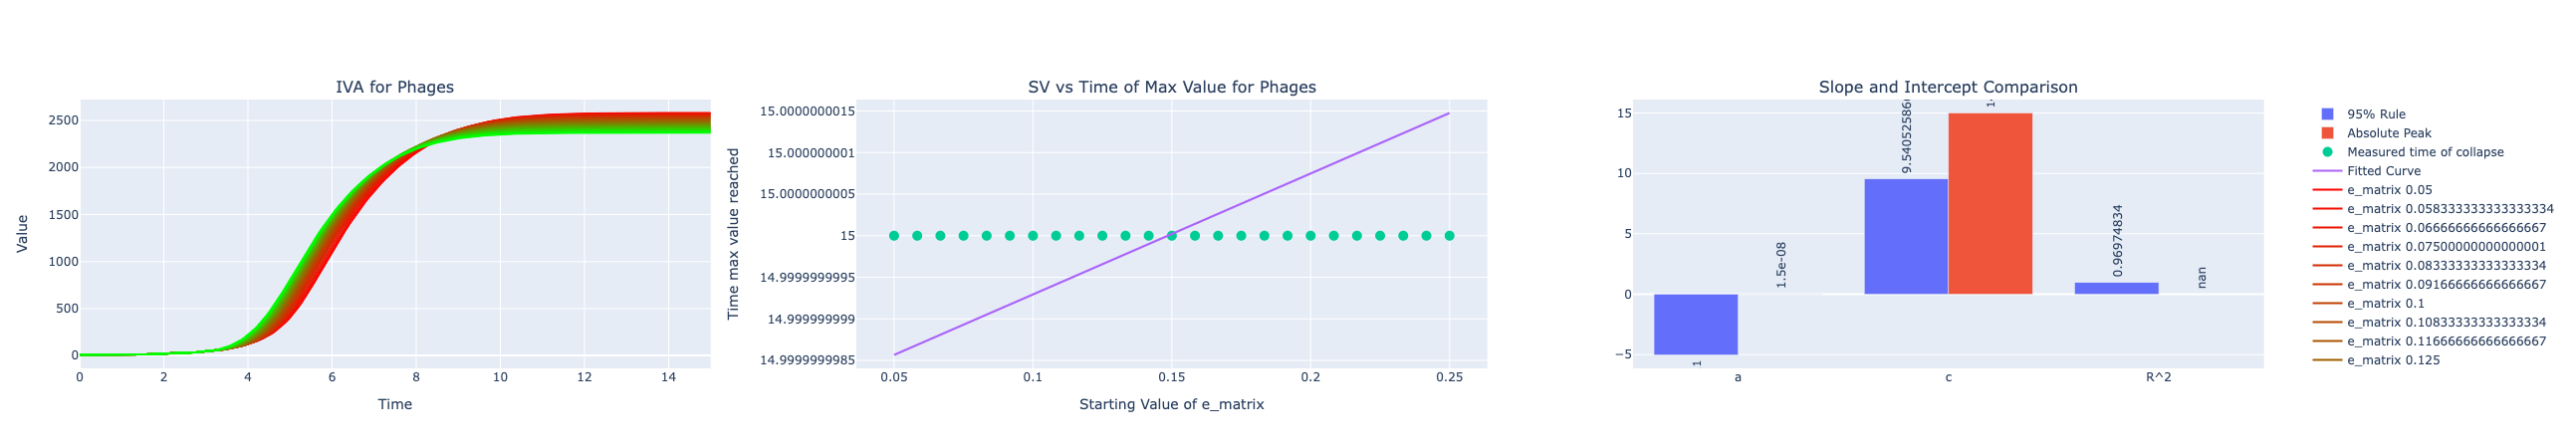
\includegraphics[width=\linewidth]{Plots/Created/IVA/initial_value_analysis_Phages_100.png}
        \caption{
            IVA for phage population, 100\% rule.  
        }
        \label{fig:appendixF:IVA_phages_100}
    \end{subfigure}
    \hfill
    \begin{subfigure}{1\linewidth}
        \centering
        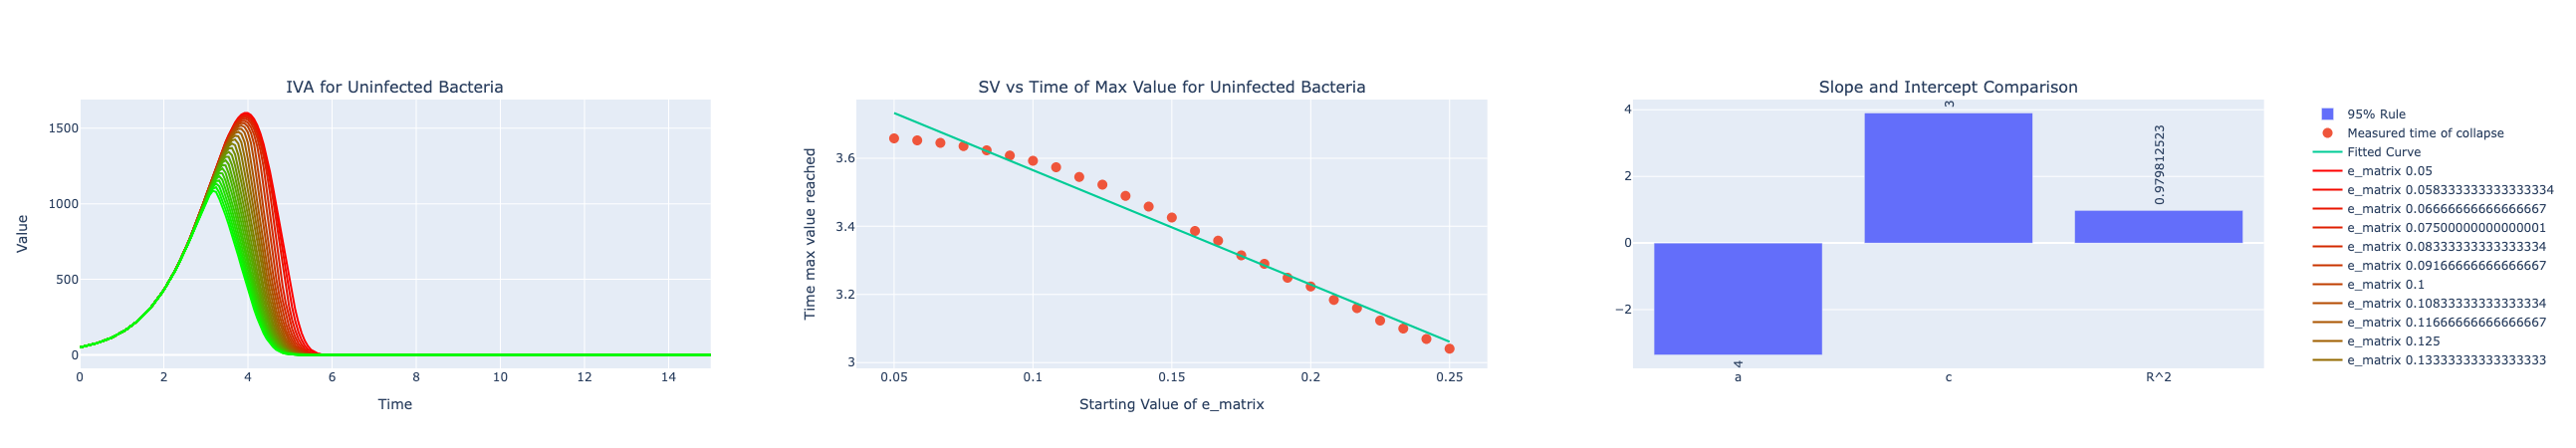
\includegraphics[width=\linewidth]{Plots/Created/IVA/initial_value_analysis_Uninfected_Bacteria_95.png}
        \caption{
            IVA for uninfected population, 95\% rule. 
        }
        \label{fig:appendixF:IVA_uninfected_bacteria_95}
    \end{subfigure}
    \hfill 
    \begin{subfigure}{1\linewidth}
        \centering
        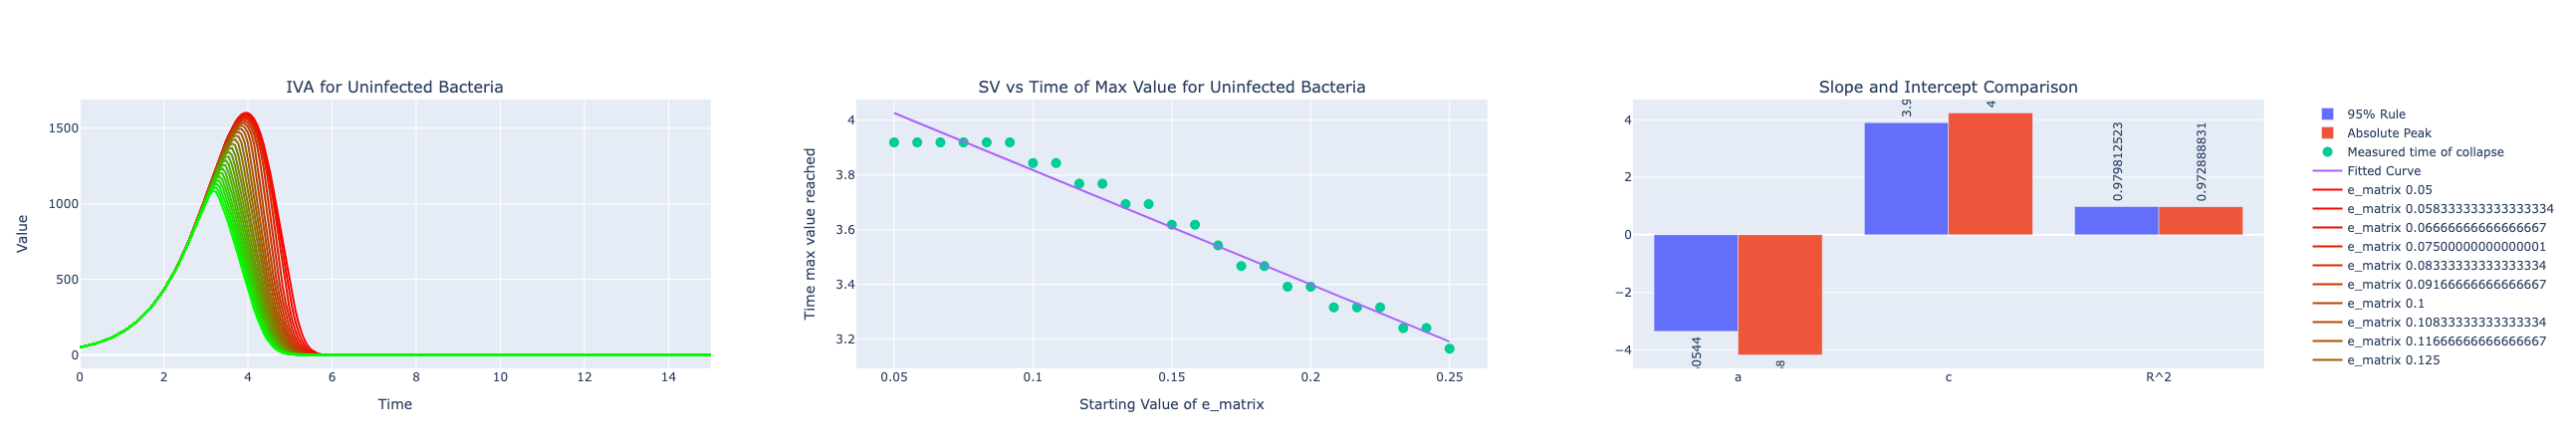
\includegraphics[width=\linewidth]{Plots/Created/IVA/initial_value_analysis_Uninfected_Bacteria_100.png}
        \caption{
            IVA for uninfected population, 100\% rule. 
        }
        \label{fig:appendixF:IVA_uninfected_bacteria_100}
    \end{subfigure}
    \begin{subfigure}{1\linewidth}
        \centering
        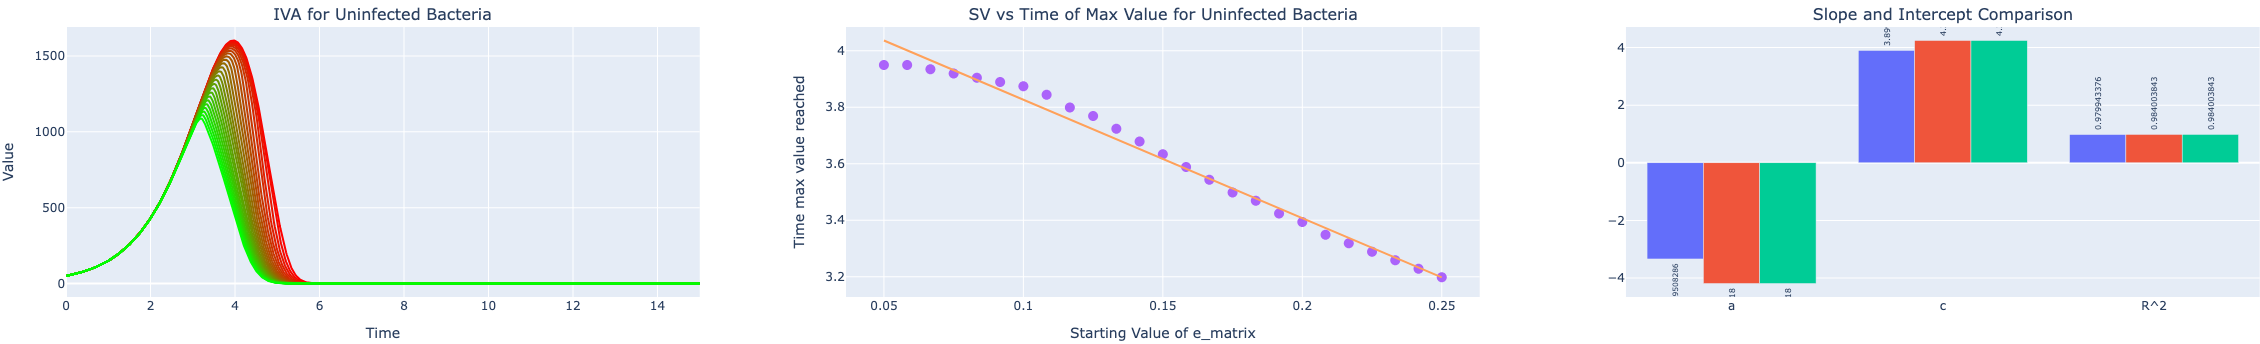
\includegraphics[width=\linewidth]{Plots/Created/IVA/initial_value_analysis_Uninfected_Bacteria_100_own_time.png}
        \caption{
            IVA for uninfected population, 100\% rule, 1000 equidistant time steps. 
        }
        \label{fig:appendixF:IVA_uninfected_bacteria_100_own_time}
    \end{subfigure}
    \caption{
        Testing the 95\% rule vs the 100\% rule, where the time at the absolute peak is taken and plotted in the second plot. 
        A comparison of phages and uninfected bacteria is shown. 
        Verification of the graph shape between the 95\% rule graph and a frequent time step with 100\% rule can be seen between c) and e). 
        The $e$ value is changed, ranging from 0.05 to 0.25. 
    }
    \label{fig:appendixF:IVA_95_vs_100}
\end{figure}

\section{Varying $r$ and $\beta$ In A $3\times 2\times 3$ System}
\Cref{fig:created:r_beta_washout_0}, \Cref{fig:created:r_beta_washout_0.02}, and \Cref{fig:created:r_beta_washout_0.05} show a 7x7 matrix of figures, each with a unique parameter set. 
In each sub-figure, the values of $r$ and $\beta$ are varied as follows: $r = 0.5, 1.1, 1.7, 2.3, 2.9, 3.5,$ inf; $\beta = 0, 20, 40, 60, 80, 100,$ inf. 
"inf" in the figures, represented as \textit{np.inf} in the code, the representation of $\infty$,  represents the original parameter values used in the IC, vector data, or matrix data. 
Each figure shows the effect of varying the washout rate, with values set to 0, 0.02, and 0.05, respectively.
All initial phage values were set to 10. 
This was done to really show how the different interactions with the bacteria, and the value of the parameters affected the phage growth. 
The default values for the parameters can be found in \Cref{tab:appendixE:complex_model}. 
\begin{figure}[]
    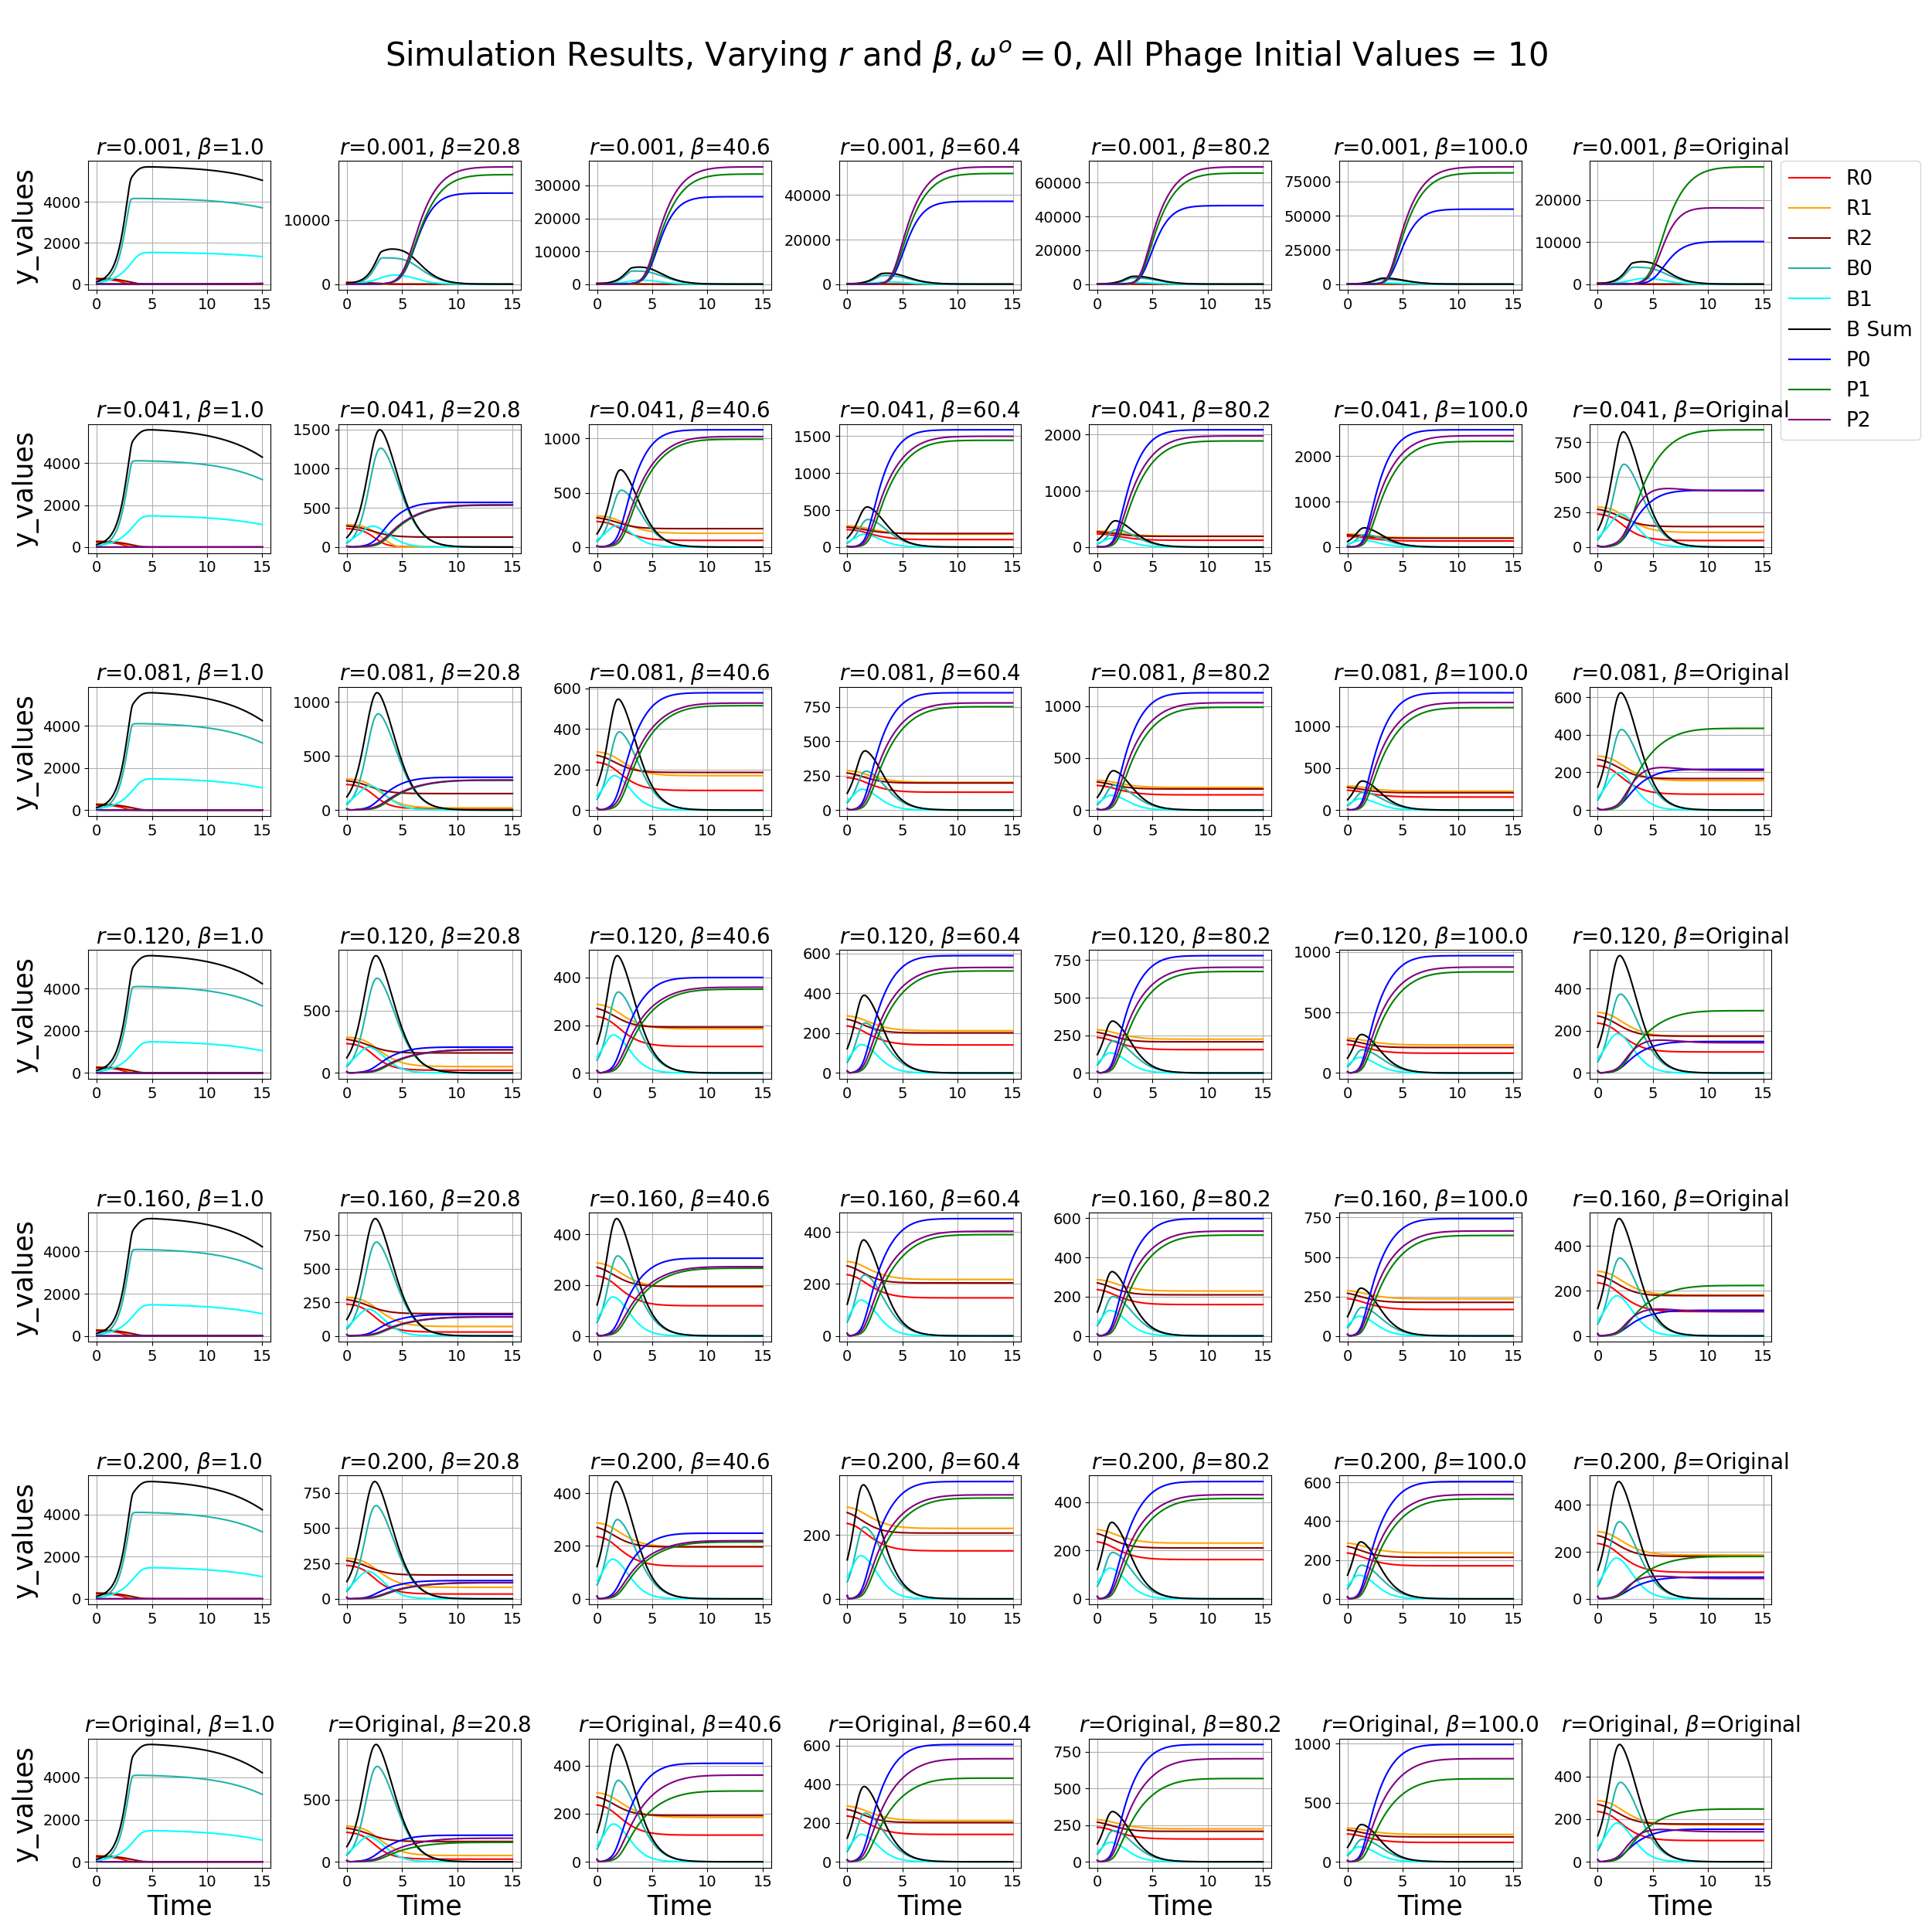
\includegraphics[width=1\textwidth]{Plots/Created/UA/r_beta_washout_0.png}
    \centering
    \caption{
        Washout $\omega^o=0$. 
    }
    \label{fig:created:r_beta_washout_0}
\end{figure}

\begin{figure}[]
    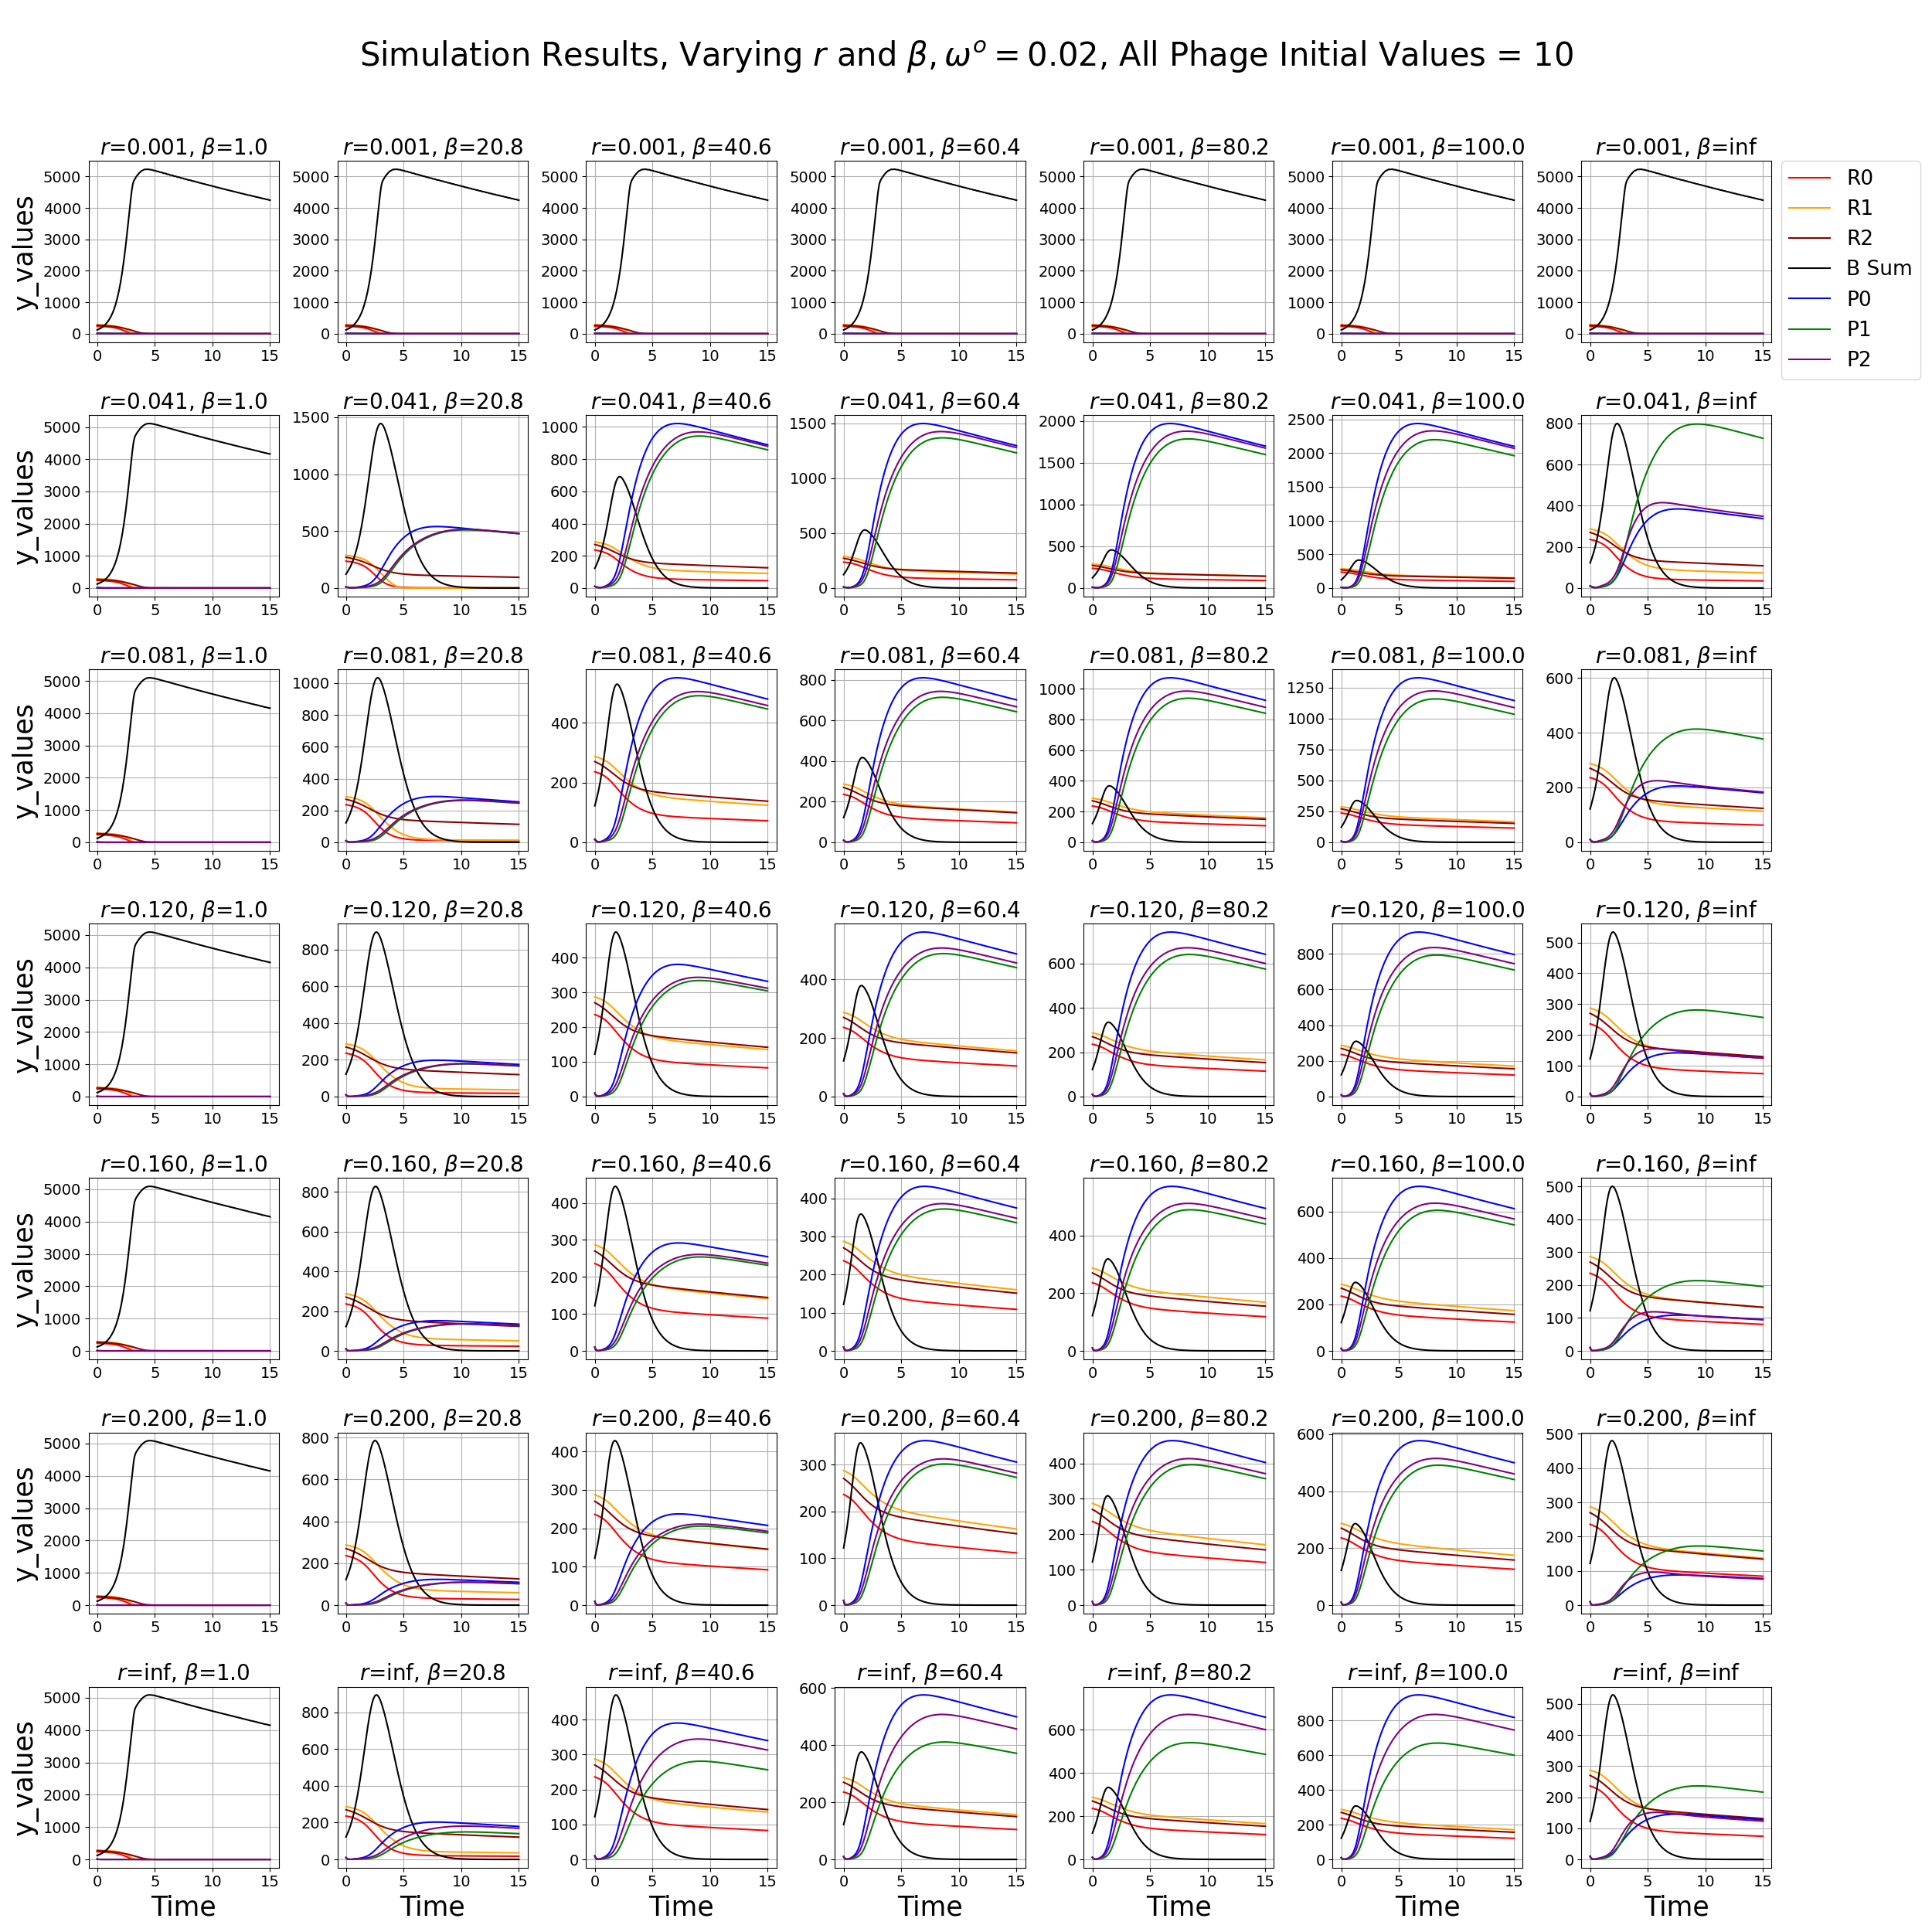
\includegraphics[width=1\textwidth]{Plots/Created/UA/r_beta_washout_0.02.png}
    \centering
    \caption{
        Washout $\omega^o=0.02$. 
    }
    \label{fig:created:r_beta_washout_0.02}
\end{figure}

\begin{figure}[]
    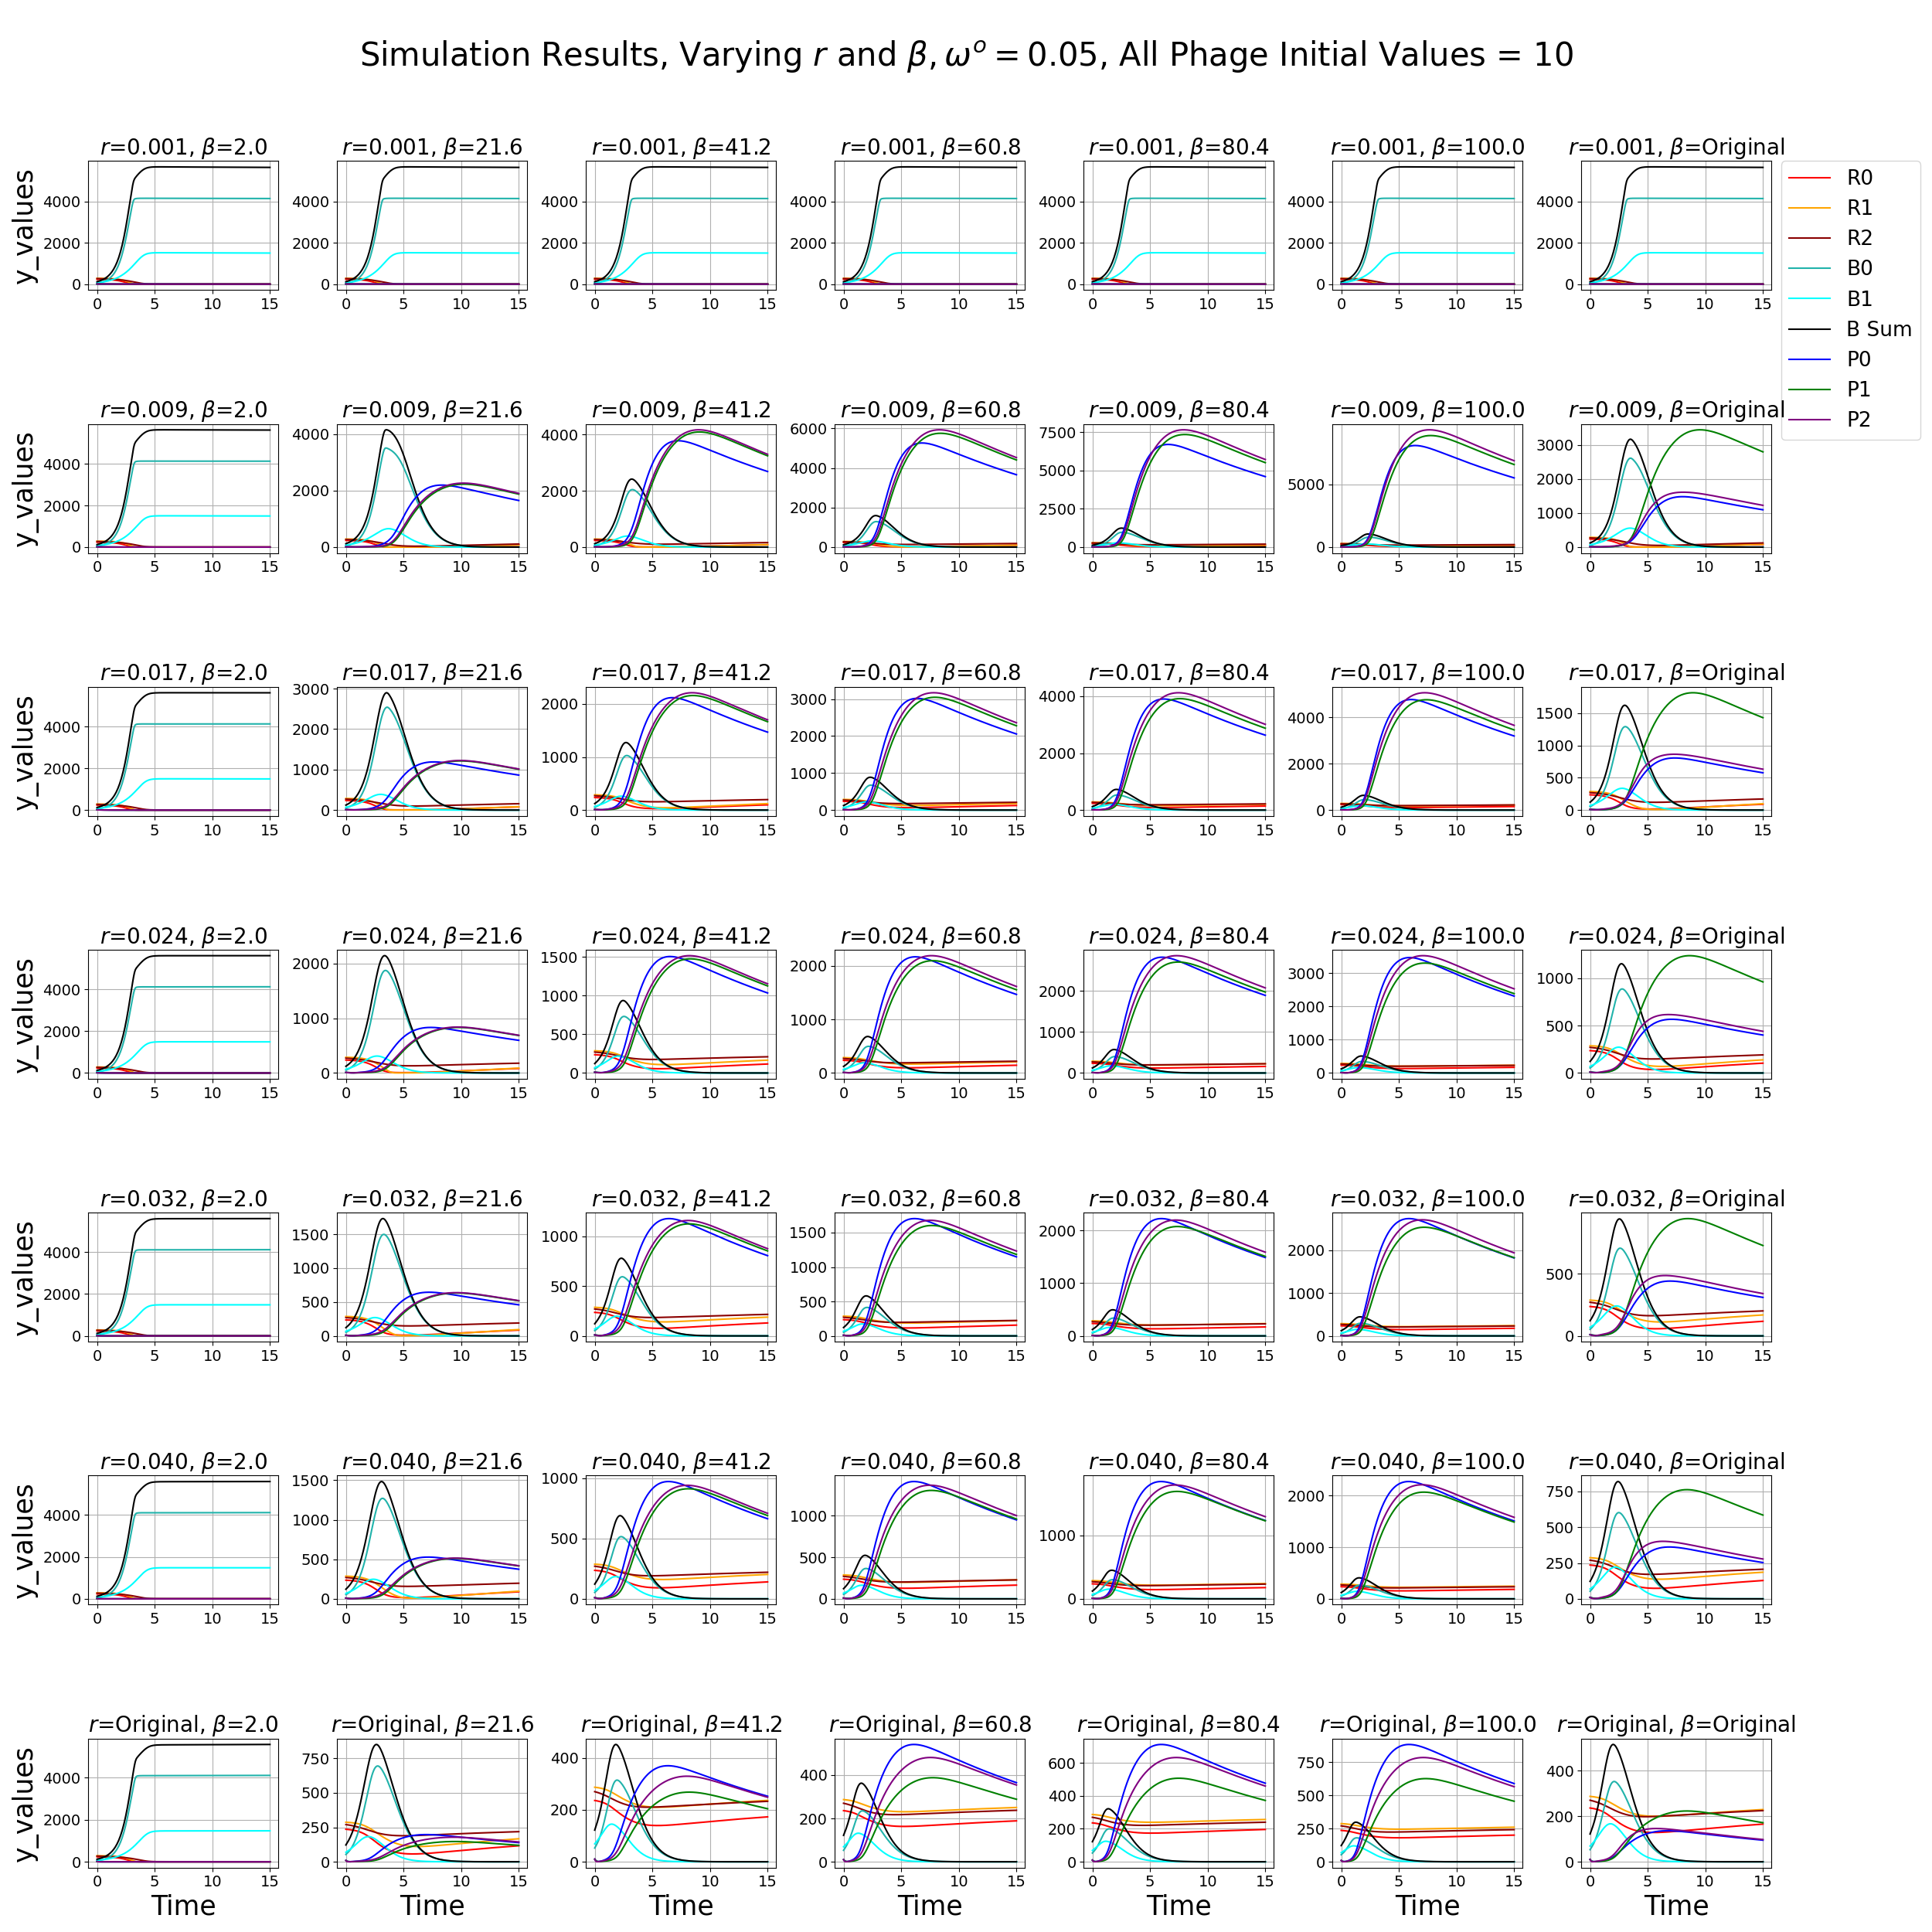
\includegraphics[width=1\textwidth]{Plots/Created/UA/r_beta_washout_0.05.png}
    \centering
    \caption{
        Washout $\omega^o=0.05$. 
    }
    \label{fig:created:r_beta_washout_0.05}
\end{figure}